\section{The data}

	\subsection{Zernike coefficients dataset}
			A dataset of 1000 zernike coefficients is created for this report.In particular, each datapoint represent the coefficients of the first 2 Zernike modes, their values ranging between [-2, -1.8] and [1.8, 2].\\
		
	\subsection{PSFs coefficients dataset}
		
		A dataset of 1000 PSFs is created using the Zernike coefficients dataset.\\
		
		\begin{figure}[ht!]
			\centering
			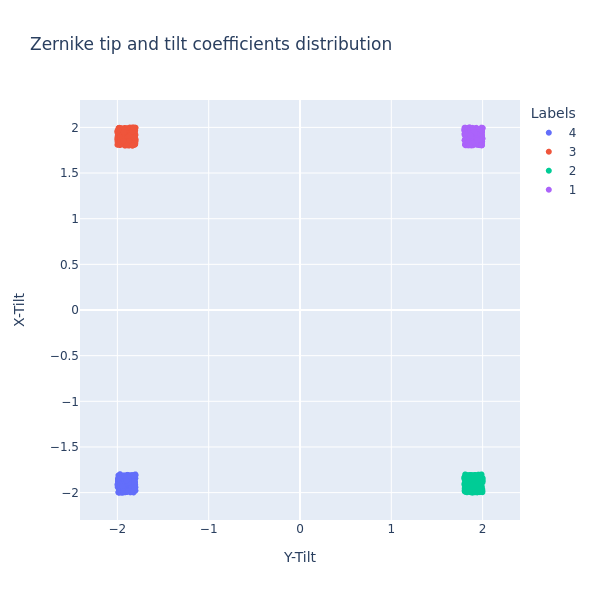
\includegraphics[width=0.4\textwidth]{mdid-originalclusters.png}
			\caption{Example original sized PSF}\hspace{\fill}
		\end{figure}
		
		These ranges create 4 original clusters that will be used as reference.
		
		\begin{figure*}[ht!]
			\centering
			\subfloat[Positive X-tilt and Positive Y-tilt PSF example]{%
				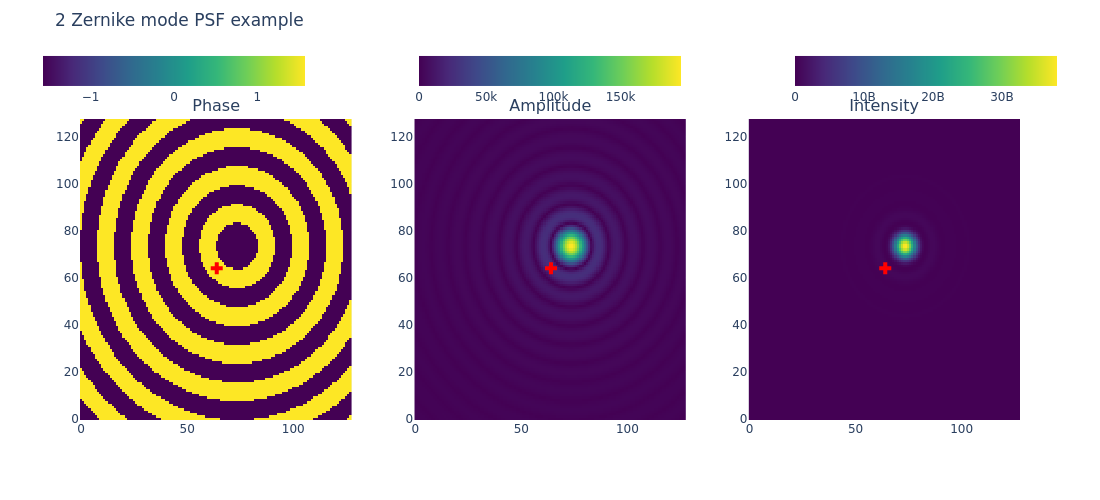
\includegraphics[width=0.6\textwidth]{mdid-ppexample}}\\
					
			\subfloat[Negative X-tilt and Positive Y-tilt PSF example]{%
				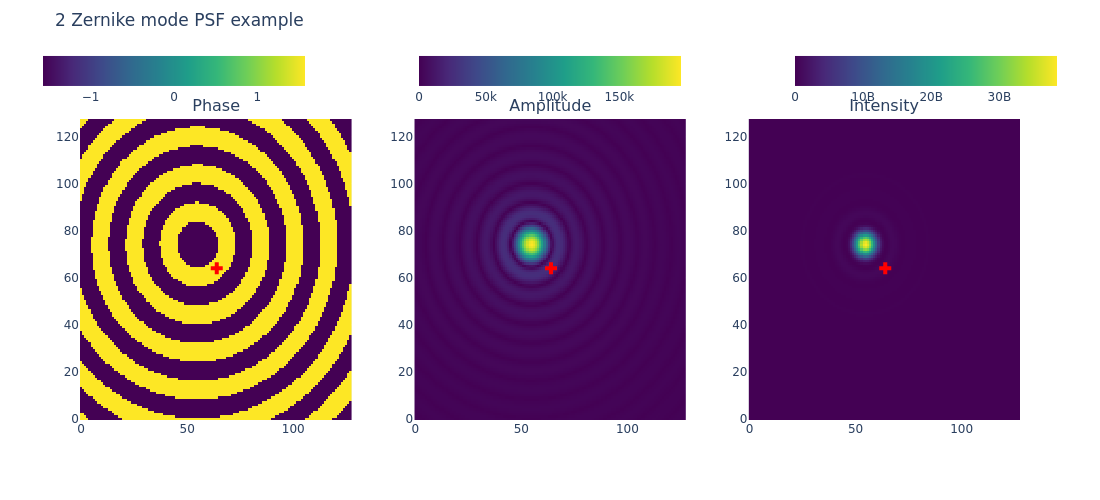
\includegraphics[width=0.6\textwidth]{mdid-pnexample}}\\
					
			\subfloat[Positive X-tilt and Negative Y-tilt PSF example]{%
				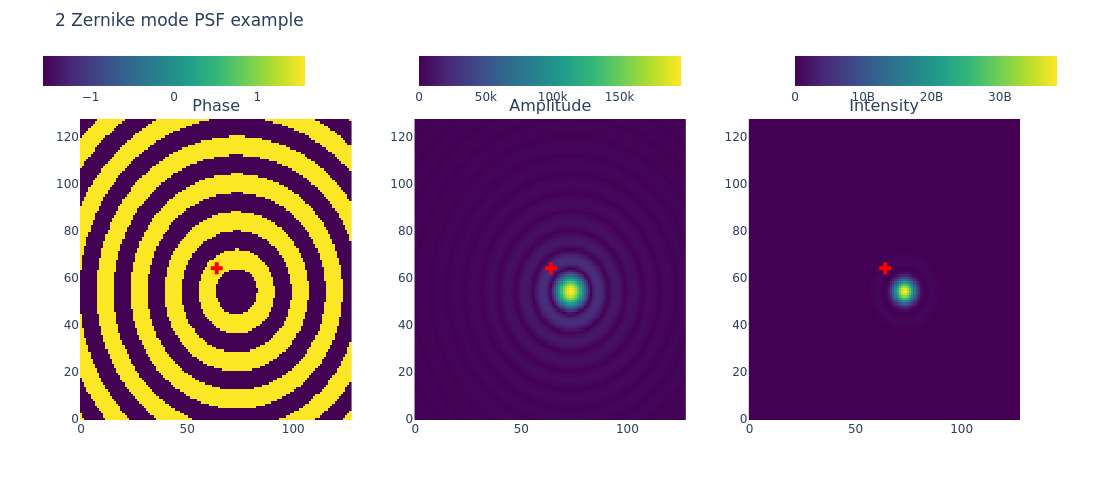
\includegraphics[width=0.6\textwidth]{mdid-npexample}}\\
					
			\subfloat[Negative X-tilt and Negative Y-tilt PSF example]{%
				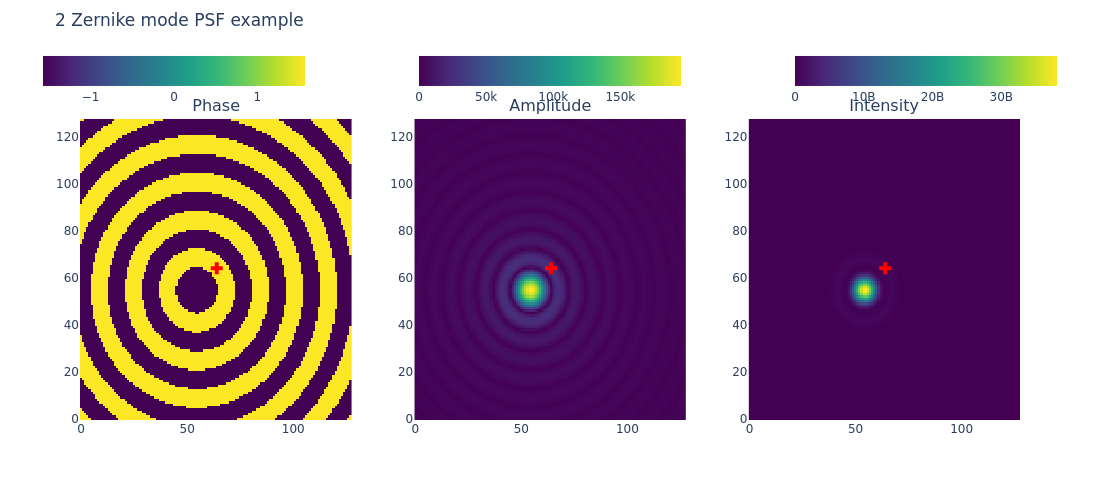
\includegraphics[width=0.6\textwidth]{mdid-nnexample}}\\
			\caption{2 Zernike modes PSF examples}
		\end{figure*}
		
		\FloatBarrier
		
	\subsection{LP mode coefficients dataset}
		A dataset of 1000 LP mode coefficients obtained from computing the overlap integral of the first 19 LP modes with the PSF dataset.
		
	\subsection{LP mode coefficients dataset}
		A dataset of 1000 PL output fluxes obtained from the PL transfer matrix and LP coefficients.
		